\customsection{Serverless backend}

Durante el desarrollo del \textit{backend} se evaluó la posibilidad de utilizar las alternativas de nube más reconocidas y con mayor facturación en el mercado actual; Lo anterior con el objetivo de implementar el desarrollo con el proveedor más confiable. Dentro de los posibles proveedores se evaluaron superficialmente las siguientes opciones: Amazon Web Services, Google Cloud y Microsoft Azure. Con una primera mirada se pudo observar que los factores diferenciadores de cada proveedor dependian estrictamente de los productos adicionales que estos podian ofrecer.
\vspace{0.5cm}\\
Por una parte, los servicios de nube de Amazon Web Services representan la mayoría del mercado de la nube, pero esto se debe en su mayoría al almacenamiento de información, por ende, tiene una gran variedad de servicios de nube, incluyendo sus tiendas en linea y sus servicios de storage webs. En resumen, su especialidad es el servicio de almacenamiento. Teniendo esto en mente, resulto una tentativa debido a la necesidad de nuestro proyecto de almacenar información de muchos dispositivos.
\vspace{0.5cm}\\
Por otra parte, los servicios de Google incluyen el uso de su red privada que tiene el mejor desempeño en velocidad dentro del mercado. En adición, los servicios de Google Cloud poseen interfaces de administración con más experiencia de usuario y la posibilidad de acceder a servicios clave para proyectos como este como el bróker serverless de IOT.
\vspace{0.5cm}\\
Finalmente, Microsoft Azure es el servicio de nube con la posibilidad de integrarse de la mejor manera con desarrollos .Net, lo anterior debido a que es la tecnología de desarrollo creada y administrada por Microsoft.
\vspace{0.5cm}\\
Cabe aclarar que al escoger a cualquiera de estos proveedores no resulta comprometido el uso de los servicios de otros: para integrar servicios de otro proveedor, solo se requiere establecer las condiciones apropiadas para autenticar nodos de red diferentes a los de las redes internas que los proveedores ya administran.
\vspace{0.5cm}\\
Teniendo en cuenta todo lo anterior se escogió el servicio de nube de Google, principalmente porque poseía la implementación del bróker de Mqtt más apropiada para el desarrollo de un proyecto de estas características. Además, el servicio de Google permitiría utilizar herramientas propias como su interfaz de procesamiento de voz natural, en el momento que se extienda el alcance del proyecto.
\vspace{0.5cm}\\
Una vez escogida la plataforma de nube y el servicio de comunicación se decidió desarrollar el \textit{backend} tipo serverless para aprovechar todas las ventajas del servicio escalable de mensajes de internet de las cosas de Google llamado ``Cloud Iot''.

\subsection{Especificaciones técnicas}

Para el montaje de la arquitectura de la nube se utilizaron principalmente 4 componentes: la base de datos MySql, el servicio de almacenamiento por contenedores tipo ``Storage 3'' de Amazon, el servicio de Cloud IOT para como bróker de internet de las cosas y las ``Cloud Functions'' de su arquitectura de nube. De los elementos anteriormente mencionados se puede entender el sistema como una serie de funciones que son activadas con eventos tipo solicitudes Https y mensajes basados en Mqtts, por ende todo el flujo de información será orquestado por las funciones que se definan en el sistema. Un diagrama generalizado se puee ver en el capitulo de introducción en la figura \ref{diagramaGeneralizado}. 
\vspace{0.5cm}\\
Las funciones de nube de Google operan como scripts de lenguajes de programación como Node.js, Python y Golang; estas requieren de librerías para operar de manera efectiva con cualquier componente del sistema. Para el desarrollo de esta arquitectura se decidió utilizar el entorno de desarrollo de Node.js, Por ende para poder hacer uso de los componentes necesarios para implementar la arquitectura planeada se utilizaron las siguientes librerías:

\begin{itemize}
	
	\item \textbf{``@Google-cloud/storage'':} Esta librería es desarrollada y mantenida por google y permite hacer uso de las descargas, las subidas y la administración de los servicios de almacenamiento de archivos ``Cloud Storage''.
	
	\item \textbf{``Mysql'':} La librería oficial de MySql para Node.js, con esta librería se implementó la comunicación con la base de datos MySql y se crearon todas las rutinas para guardar y obtener datos en la base de datos.
	
	\item \textbf{``Googleapis'':} Esta librería es la encargada de comunicarse directamente con cualquier dispositivo conectado a la red, fue utilizada para reenviar los mensajes recibidos por los dispositivos a través del puente ``Cloud Iot''.
	
	\item  \textbf{``Jsonwebtoken''} Esta librería fue utilizada para autenticar los mensajes recibidos por las solicitudes Https y Mqtts, a partir de las llaves públicas de los dispositivos registrados en el sistema. El algoritmo de encriptación utilizado fue el RSA256.
	
	\item  \textbf{``Google-auth-lib''} La librería de autenticación de google fue utilizada para obtener las credenciales necesarias para utilizar el puente de Iot del proyecto.
	
\end{itemize}


\subsection{Base de datos relacional y no relacional}

Una parte muy importante de la arquitectura es la base de datos y, aunque el sistema de almacenamiento de ``Cloud Storage'' funciona como un disco duro con todas las facilidades para majear archivos naturales, tiene limitaciones y costos asociados al número de operaciones de lectura y escritura que se pueden hacer en el mes. Por el contrario, la base de datos MySql tiene costos asociados únicamente con el tamaño del almacenamiento y la capacidad del procesador; debido a esto es la opción más apropiada para almacenar datos de pequeño tamaño pero de gran cantidad es la base de datos relacional MySql.
\vspace{0.5cm}\\
El diseño de la base de datos estuvo apoyado por el programa de administración de bases de datos: \textsl{``MySql Workbench''}. Un esquema generalizado de la base de datos se puede observar en el diagrama \ref{fig_23}, donde cada cuadro representa un grupo de tablas bajo el paradigma SQL. 
\vspace{0.5cm}\\

\begin{figure}[htbp]
	\centerline{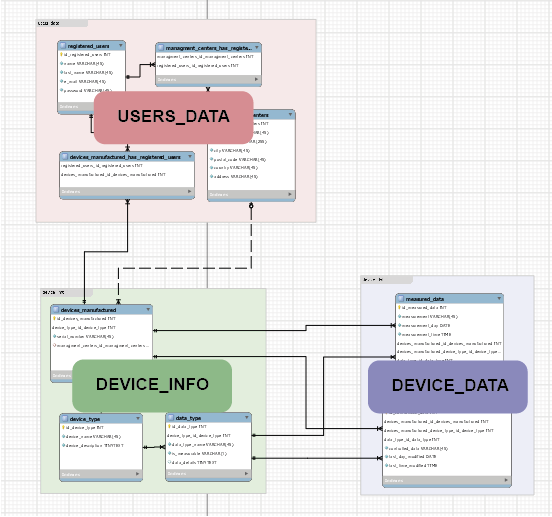
\includegraphics[width=14cm]{figuras/UML.png}}
	\caption{Diseño de las tablas de la base de datos relacional MySql. Fuente: propia}
	\label{fig_23}
\end{figure}

Teniendo en cuenta lo anterior, se explicará por separado cada grupo de tablas con el objetivo de mostrar las escalabilidad del sistema y como fue implementada la base de datos pensando en los requerimientos funcionales de los productos House Manger y User App. cabe aclarar que para representar los tipos de columnas se utilizaron los siguientes símbolos: un bombillo amarillo significa que se trata de una columna de llave primaria única, un rombo azul representa un buffer de tipo \textit{char} obligatorio, un rombo blanco significa buffer de tipo \textit{char} no obligatorio y las columnas sin símbolo son llaves secundarias de relación obligatorias.


\begin{itemize}
	
	\item \textbf{Users data:} En este grupo de tablas se encuentran principalmente 2 tablas:
	\vspace{0.5cm}\\
	La tabla registered\_users, que almacena la información de los clientes; esta información consta de un correo de registro y un espacio para la ``contraseña''. Realmente el espacio de la contraseña es una entrada para una ``llave privada'' generada por Google que se utiliza para acceder a la información personal de los usuarios desde el \textit{backend}. 
	\vspace{0.5cm}\\
	La tabla managment\_centers, que agrupa los dispositivos fabricados en regiones de operación; en esta tabla se tiene como objetivo referenciar a los usuarios y los dispositivos a una zona horaria GTM y una descripción de dirección. En el caso de realiza envíos o referenciar espacios geográficos esta tabla presenta una utilidad más representativa.
	\vspace{0.5cm}\\
	Finalmente, Las tablas adicionales son las tablas de relación muchos a muchos de un paradigma SQL relacional.
	
	\begin{figure}[htbp]
		\centerline{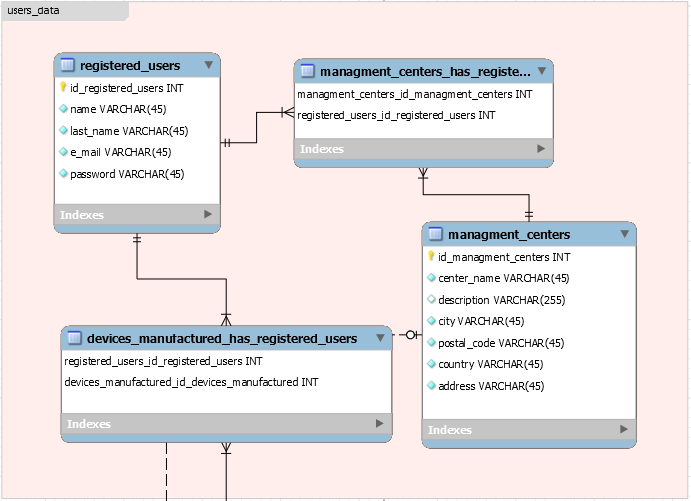
\includegraphics[width=7cm]{figuras/users_data.png}}
		\caption{Grupo de tablas: users data. Fuente: propia}
		\label{fig_25}
	\end{figure}
	
	\item \textbf{Device\_info:} En este grupo existen 3 tablas y todas contienen información relevante: La tabla devices\_manufatured contiene principalmente el número serial. La tabla device\_type contiene una breve descripción del dispositivo y su nombre. Por último, la tabla  data\_type sirve para almacenar la información de todas las posibles variables medibles y los actuadores configurables para todos los dispositivos. Teniendo en cuenta que el sistema puede recibir dispositivos que no han sido fabricados de manera propia, juntando el nombre y el numero serial, se obtiene una identificación única por sensor o actuador conectado al sistema. 
	
	\begin{figure}[htbp]
		\centerline{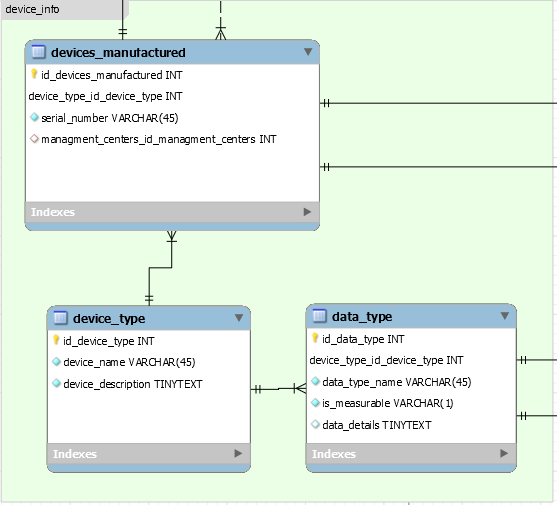
\includegraphics[width=7cm]{figuras/device_info.png}}
		\caption{Grupo de tablas: device info}
		\label{fig_26}
	\end{figure}
	
	\item \textbf{Device\_data:} El grupo de tablas de información se compone únicamente de 2; la tabla measured\_data contiene únicamente la información que fue medida y tiene una estampa de tiempo de mínimo 1 segundo, la tabla controllable\_data contiene las estampas de tiempo en las cuales se le dio la orden al dispositivo modificar su actuador de forma específica. Teniendo en cuenta lo anterior, un valor de control en un momento especifico no garantiza que ese actuador se haya modificado de esa forma en el centro de gestión; garantiza que el dispositivo estaba conectado a la red y recibió el comando de hacerlo.
	
	\begin{figure}[htbp]
		\centerline{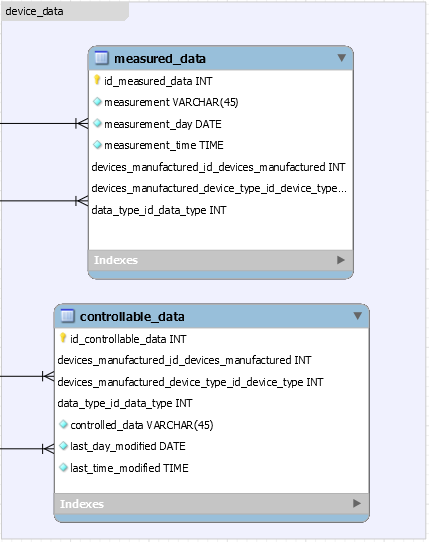
\includegraphics[width=7cm]{figuras/device_data.png}}
		\caption{Grupo de tablas: device data. Fuente: propia}
		\label{fig_27}
	\end{figure}
	
\end{itemize}

Finalmente el componente no relacional del sistema de almacenamiento tipo ``Storage 3'' funciona como un sistema de archivos y tiene como interfaz la api propia de google anteriormente mostrada. Internamente para almacenar la información de los usuarios se organizó la información en carpetas con el nombre ``sql\_uid{id mysql}'' donde el texto ``{id mysql}'' corresponde a la llave primaria única entera utilizada para identificar a los usuarios en la base de datos relacional (la columna llamada ``id\_registered\_users'' de la tabla ``registered\_users'')
\vspace{0.5cm}\\
Teniendo en cuenta la estructura de almacenamiento anteriormente mencionada, el sistema obtiene su cuello de botella en el número de conexiones MySql que puede recibir, todos los demás elementos pueden escalar, en teoría, de manera infinita. Para la versión de la base de datos que se está utilizando se pueden permitir 4000 conexiones simultaneas, por ende, se dice que el sistema está diseñado para 4000 usuarios.

\subsection{Relación de requerimientos funcionales}

Debido a que este producto no se contempló en la estaba de conceptualización y planeación del proyecto no tuvo una lista de requerimientos funcionales sobre los cuales crear scripts o funciones, por el contrario, los requerimientos funcionales de los otros dos productos: El House Manager y el User Manager exigían un desarrollo desde la perspectiva del \textit{backend}. Teniendo en cuenta lo anterior, se explicaran los desarrollos realizados en el \textit{backend} y los requerimientos funcionales que pretendían solucionar.

\begin{enumerate}
	\item \textsl{``El usuario debe poder acceder a la información medida en tiempo real''.} Para cumplir este objetivo fue necesario crear un puente de conexión en tiempo real de un dispositivo a otro, siendo el segundo un dispositivo de monitoreo como lo es la User App. El puente es realizado por el “cloud iot” y a travez de una función de nube que es activada cada vez que se reporta un valor de medición (esta función será explicada más adelante)
	\item \textsl{``El usuario debe poder acceder al histórico del mes y la relación de sus gastos con ellos''.} Como solución a este requerimiento se diseñó una REST API (aquel conjunto de funciones basadas en solicitudes Http, que se utilizan para ofrecer un servicio en específico) capaz de obtener datos de la base de datos de medición o control entre un periodo de tiempo específico. 
\end{enumerate}


\subsection{Funciones de nube}
Las funciones de nube implementadas tienen como características: una memoria ram de 512 megabytes, la posibilidad de tener acceso a una memoria volátil temporal únicamente existente durante el tiempo de ejecución de la función y la posibilidad de ejecutar los lenguajes de programación: Node.js, Python y Go. Cabe aclarar que este tipo de arquitectura posee como limitación un límite de ejecución por función de 9 minutos.
\vspace{0.5cm}\\
Teniendo en cuenta lo anterior y los requerimientos funcionales se implementaron 4 funciones de nube que serán explicadas en los siguientes apartados.

\subsubsection{Get\_historical\_data:}

Esta función fue diseñada para recibir un mensaje a través de un ``post request''. El contenido del post debe ser buffer codificado a 64 bits con un objeto de JavaScript (Json) convertido. El contenido de este objeto debía ser el necesario para: validar la legitimidad de la solicitud, conocer el tipo de dato que se desea obtener de la base de datos, el dispositivo del cual se desea conocer la información y el rango de tiempo en el que se desean consultar los datos. Teniendo en cuenta lo anterior un ejemplo del objeto Json aceptado como argumento de la función es:
\begin{Verbatim}[tabsize=4]
{
	"type":"control",
	"sql_uid":1,
	"number_points": 10,
	"device_name": "House Manager SDL"
	"serial_number": 1000023211
	"data_type": "potencia activa instantanea",
	"init_date": "2019-07-18",
	"final_date": "2019-08-12",
	"encripted_token": "SsidfmjEFShfDBGSsdEFSBzdfw3RQEfassdg23"
}
\end{Verbatim}
Donde  el campo ``type'' es opcional y tiene como valor por defecto los datos de medición, el campo ``sql\_uid'' corresponde al identificador único de usuario de la base de datos, el campo ``number\_points'' corresponde al número máximo de puntos que puede tener el objeto de respuesta, ``serial\_number'' es el numero serial del dispositivo que genero los datos que se desean obtener, ``data\_type'' es un string con el nombre del tipo de dato registrado en la tabla data\_type, los campos ``init\_date'' y ``final\_date'' representan los límites temporales en los cuales se debe realizar la consulta.
\vspace{0.5cm}\\
Por último, el campo ``encripted\_token'' se debe incluir un Sting encriptado conteniendo el objeto de autenticación. El Sting debe estar encriptado utilizando el algoritmo de Rivest–Shamir–Adleman de 256 bits y el objeto descifrado debe contener la siguiente información:

\begin{Verbatim}[tabsize=4]
{
	iat: 1234232009,
	exp: 1236323009
}
\end{Verbatim}


Donde ``iat'' es un entero con el número de milisegundos en los cuales se creó el token, teniendo en cuenta, un punto de referencia de la maquina (Enero 1 de 1970 a la hora 00:00:00 UTC.) y el campo ``exp'' es también un entero con los milisegundos en los cuales expira el token, de autenticación, teniendo en cuenta el mismo punto de referencia.
\vspace{0.5cm}\\
Debido a que el sistema de autenticación basado en los JWT es el mismo en todas las funciones no será explicado nuevamente en las siguientes secciones, solo serán explicados los campos nuevos o los que tengan un significado diferente.
\vspace{0.5cm}\\
El algoritmo de la función se puede separar en 5 pasos generales, fig \ref{fig_28}, cada uno de los pasos se puede ver a continuación:
\begin{figure}[htbp]
	\centerline{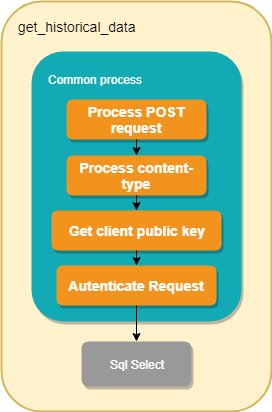
\includegraphics[width=6cm]{figuras/algoritmo_get_historical.png}}
	\caption{Algoritmo de la función: Get historical data. Fuente: propia}
	\label{fig_28}
\end{figure}
\begin{enumerate}
	\item \textbf{Segmentacion del tipo de request:} En esta etapa de la función se verifica que la solicitud sea unicamente de tipo POST
	\item \textbf{Segmentacion por formato de mensaje:} En esta etapa se verifica que el tipo de contenido del mensaje sea ``application/json''
	\item \textbf{Adquisicion de la llave publica:} Para autenticar el usuario se accede al servicio de almacenamiento S3 para optener la llave ``verificadora'' del usuario en cuestión.
	\item \textbf{Autenticación de usuario:} Se descifra el token de acceso y se verifica que el token no se encuentre vencido.
	\item \textbf{Consulta SQL:} Se utiliza la información contenida en el mensaje para realizar una consulta SQL dependiendo del tipo de operación y se organizan los datos en un objeto resultado.
\end{enumerate}
Teniendo en cuenta el proceso anterior, un ejemplo del objeto resultante de solicitud Http a esta función es:

\begin{Verbatim}[tabsize=4]
{
	``data\_type'': ``potencia activa instantanea,
	"data": [
		{
			"data": "1213123",
			"date": "2019-06-12",
			"time": "17:44:51",
		},
		{
			"data": "333123",
			"date": "2019-07-12",
			"time": "3:12:11",
		}
	]
}
\end{Verbatim}
Donde el objeto es un Json codificados en base 64 del objeto convertido a Sting. el contenido de "data" depende del número de puntos que se soliciten y el campo "data\_type". Teniendo en cuenta el vector de datos de ejemplo, cabe aclarar que toda la información temporal recibida esta referenciada a la zona horaria cero (UTC: 0).

\subsubsection{Send\_command:}

Esta función también fue diseñada para recibir un mensaje a través de un "post request". y también debe recibir un buffer codificado a 64 bits con un objeto de JavaScript (Json) convertido. La razón por la cual se escogió el "POST" como el tipo de solicitud fue puesto que con las solicitudes post el servidor en cuestión encripta la información usando su certificado de seguridad SSL, es decir, que en este caso la información transmitida esta encriptada con el certificado SSL de Google.
\vspace{0.5cm}\\
Teniendo en cuenta que la función también fue diseñada basada en un post y con todos los requerimientos de encriptación y codificación, un ejemplo de un mensaje seria:
\begin{Verbatim}[tabsize=4]
{
	"sql_uid": 1,
	"mqtt_sub_folder": "control/raspberry",
	"operation": "send-save",
	"encripted_token": "SsidfmjEFShfDBGSsdEFSBzdfw3RQEfassdg23",
	"message":{
		"some_json_object"
	}
}
\end{Verbatim}
Dado el anterior objeto Json: el campo de ``mqtt\_sub\_folder'' define el tema al cual el dispositivo  de recepción está suscrito. El campo ``operation'' contiene una de las siguientes opciones; send-save, send o save y controla la operación que debe realizar el \textit{backend} con el mensaje. En caso de ser save, solo guardará en la base de datos el mensaje enviado (este mensaje debe contener la información necesaria para guardarse en la base de datos; si no tiene el formato indicado, no será guardado en la base de datos a pesar de que si sea enviado y recibido por el dispositivo). En caso de solo ser send, el \textit{backend} le enviara un mensaje al dispositivo, si es posible, y finalizara la operación. Finalmente, si la operación es send-save el \textit{backend} intentará enviarle un mensaje al dispositivo, si lo recibe, asume que la variable de control fue modificada y guarda en mensaje en la base de datos.
\vspace{0.5cm}\\
El campo message contiene el mensaje que recibirá el dispositivo, teniendo en cuenta que el mensaje es para la modificación de una variable de control el mensaje debe contener la estampa de tiempo en la que se generó la orden, el valor al cual se desea modificar la variable y el tipo de data a la cual corresponde la información. Un ejemplo de Json con la capacidad para almacenar la información de la orden es:
\begin{Verbatim}[tabsize=4]
"some_json_object" = {
	"device_name": device_name,
	"serial_number": serial_number,
	"data_type": ["control circuito a", "control circuito b"],
	"data": ["off","on"],
	"date": ["2019-06-12", "2019-07-12"],
	"time": ["3:12:11", "3:12:40"],
}
\end{Verbatim}
Como se puede observar anteriormente, los campos de "data", "date" y "time" contienen un vector, lo que le permite a esta función realizar múltiples operaciones SQL y modificar múltiples actuadores con una sola solicitud.
\vspace{0.5cm}\\
El resultado de esta operación es un objeto tipo Json con la información de la operación SQL, es decir, información como el número de columnas afectadas, el tiempo que tomo la operación, entre otros. Para más información de este objeto se puede revisar la documentación oficial de la librería de mysql \cite{mysql}.
\vspace{0.5cm}\\
Adicionalmente, un diagrama generalizado del algoritmo se puede ver en la figura \ref{fig_29}. Teniendo en cuenta esta figura el algoritmo de la función se puede dividir en 6 pasos:

\begin{figure}[htbp]
	\centerline{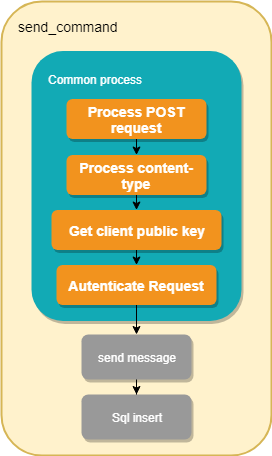
\includegraphics[width=6cm]{figuras/algoritmo_send_command.png}}
	\caption{Algoritmo de la función: Send command. Fuente: propia}
	\label{fig_29}
\end{figure}

\begin{enumerate}
	\item \textbf{Segmentación del tipo de request:} Al igual que en la función anterior se discrimina para que solo se acepten solicitudes tipo ``POST''
	\item \textbf{Segmentación por formato de mensaje:} Así como en la función ``get\_historical\_data, se rechazan las solicitudes que no tengan como formato de contenido ''application/json''.
	\item \textbf{Adquisicion de la llave publica:} También, hacemos la consulta al servicio de almacenamiento para adquirir la llave pública que será usada en el proceso e descifrado.
	\item \textbf{Autenticación de usuario:} Nuevamente Se descifra el token de acceso y se verifica que el token no se encuentre vencido.
	\item \textbf{Envío del mensaje Mqtt:} Se envía exactamente el contenido del campo mensaje al dispositivo de interés usando el tópico especificado en el campo (``mqtt\_topic'')
	\item \textbf{Registro de la información:} si el dispositivo está conectado y ha recibido correctamente el mensaje, se guarda la información del mensaje en la base de datos, si el mensaje no tiene el formato indicado este último paso no se realiza.
\end{enumerate}

\subsubsection{IOT\_gateway\_control:}

Esta función es muy diferente a las otras dos funciones explicadas anteriormente; por el contrario a ellas, esta función es activada o ejecutada a través de un sistema de publicación y suscripción interno de Google Cloud (``pub/sub message system'') para comunicar sus diferentes dependencias. En el momento que un bróker Mqtt recibe una publicación bajo el tema ``control'' un evento de pub/sub se genera, y por consiguiente, esta función de nube que está asociada a él. 
\vspace{0.5cm}\\
Adicionalmente, el proceso y funcionamiento de la función puede considerarse igual al de las otras dos funciones con pequeños cambios, todo el proceso de autenticación es manejado directamente por el servicio de ``Cloud Iot'', por ende el campo ``encripted\_token'' ya no se encuentra en los mensajes recibidos. Un ejemplo de un mensaje enviado por un dispositivo a través de una publicación Mqtt es:
\begin{Verbatim}[tabsize=4]
{
	"sql_uid": 1, 
	"mqtt_sub_folder": "control/raspberry",
	"operation":"send-save",
	"message":{
		"device_name": "House Manager SDL",
		"serial_number": 1000000000,
		"data_type": ["circuito 1","circuito 2"],
		"data": ["on", "off"],
		"date": ["2019-06-12", "2019-10-0"],
		"time": ["17:44:51", "21:00:51"],
	}
}
\end{Verbatim}
Teniendo en cuenta el Json anterior se puede observar que su formato es muy parecido al del objeto de la función ``send\_command'' con la diferencia que no contiene el campo de objeto encriptado, esto se debe a que el objeto encriptado es utilizado como contraseña al momento de establecer la conexión con el bróker desde el cliente. En adición, un diagrama generalizado del algoritmo se puede ver en la figura \ref{fig_30}. Teniendo en cuenta esta figura el algoritmo de la función se puede dividir en 4 pasos:

\begin{figure}[htbp]
	\centerline{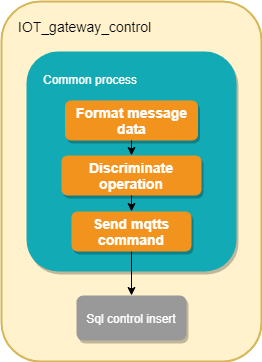
\includegraphics[width=6cm]{figuras/algoritmo_iot_control.png}}
	\caption{Algoritmo de la función: Iot gateway control. Fuente: propia}
	\label{fig_30}
\end{figure}
\begin{enumerate}
	\item \textbf{Organizar el mensaje:} Los mensajes recibidos por el broker Mqtt de Google tienen un formato tipo ``buffer'', por lo tanto, en esta etapa se convierte el arreglo recibido en un formato interpretable por el sistema.
	\item \textbf{Discriminación de operacion:} Asi como se discriminó en la funcion ``Send\_command'' en este campo se describe el tipo de operacion que se debe realizar con el mensaje. La operacion será ``send-save'' por defecto
	\item \textbf{Envío del mensaje de control Mqtt:} Se envia exactamente el contenido del campo mensaje al dispositivo de interés a travez de su tema (``mqtt topic'').
	\item \textbf{Registro de la información:} si el dispositivo está conectado y ha recibido correctamente el mensaje, se guarda la información del mensaje en la base de datos, si el mensaje no tiene el formato indicado este último paso no se realiza.
\end{enumerate}

\subsubsection{IOT\_gateway\_measure:}

Esta función comparte todos sus pasos con la anterior, es decir que es muy parecida desde una perspectiva general; la diferencia se encuentra en el último paso de la misma, un diagrama generalizado de este algoritmo se puede ver en la figura \ref{fig_31}. En el último paso, si todos los anteriores fueron completados exitosamente, el algoritmo intenta guardar la información en la tabla de control de la base de datos.

\begin{figure}[htbp]
	\centerline{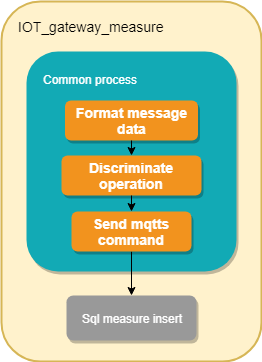
\includegraphics[width=5cm]{figuras/algoritmo_iot_measure.png}}
	\caption{Algoritmo de la función: Iot gateway measure. Fuente: propia}
	\label{fig_31}
\end{figure}

En adición, la función debe recibir un Json con el mismo formato que el recibido por ``iot\_gateway\_control'' con diferencias en sus campos: ``data\_type'' y ``mqtt\_sub\_folder'', puesto que en el tipo de dato debe contener el identificador de la variable de control y en mqtt\_sub\_folder debe haber un Sting que identifique el tópico Mqtt que el dispositivo destino pueda reconocer como un mensaje de control. 
\vspace{0.5cm}\\
Para efectos prácticos, en esta etapa de la implementación, con el objetivo de discernir un tipo de mensaje de otro se escogió como formato de tema: ``{nombre}/control'', donde {nombre} es el nombre del dispositivo al cual se le desea enviar el mensaje. Con esto, no se quiere decir que el tema Mqtt esté ligado a este formato, en el caso que se deseen escalar los comandos y añadir más actuadores a un dispositivo ya diseñado, se puede modificar el sistema de temáticas propuesto para esta versión de los productos  \textit{backend}.

